\documentclass[10pt]{article}
\usepackage[margin=0.82in]{geometry}
\usepackage{amsmath,amssymb,booktabs,tabularx,graphicx,microtype,enumitem,hyperref,xcolor,placeins}
\newcolumntype{Y}{>{\raggedright\arraybackslash}X}
\hypersetup{colorlinks=true,linkcolor=blue!45!black,urlcolor=blue!45!black,citecolor=blue!45!black}

\title{PRA-SGLang: Query-Addressed Non-Prefix Memory beside RadixAttention}
\author{Jorge Sim\~ao\\EInnovator R\&D}
\date{August 2026}

\begin{document}
\maketitle

\begin{abstract}
SGLang's RadixAttention reuses exact token prefixes. Progressive Retrieval
Attention (PRA) selects versioned non-prefix resources and intervals according
to the current query. We implement a logical PRA object namespace and an
SGLang adapter and an MLX runner-cache bridge that keeps PRA memory outside
Radix prefix accounting while consuming it as selected native K/V. A
25-request Apple-M5 smoke study with patched SGLang MLX
separates exact radix reuse from selected-memory recovery. Prefix plus selected
memory and full context both recover the fixed answer in 5/5 requests, while
the no-evidence controls are 0/5. Selection uses 365 prompt tokens instead of
1,577. The scheduler reports 364 cached tokens on warm selected requests and
1,576 on warm full-context requests; warm TTFT is 34.1 and 52.7 ms,
respectively. In a separate five-seed native-cache experiment, selected K/V
recovers 5/5 answers and is bit-exact to SGLang's ordinary split cache. All 28
attention layers consume selected memory under one normalization, while the
scheduler-visible local offset excludes every PRA token. HiCache placement and
full hierarchical placement remain open. The bridge now also runs through
SGLang's real prefill and batched-decode lifecycle: native and full context
recover 5/5, disabled memory recovers 0/5, and native throughput rises from
6.59 to 14.54 requests/s between concurrency one and eight. Shared immutable
K/V avoids 108.0 MiB at concurrency eight. Across 40 QASPER and 40 HotpotQA
natural-text transport controls per condition, native and full context are
80/80, disabled is 40/80, and shuffled memory is 32/80.
\end{abstract}

\section{Introduction}
A prefix cache and a retrieval memory answer different questions. A radix tree
asks whether token histories share an exact path. PRA asks which retained
resource or interval is useful for a query. A long-running session can use both:
\[
  \underbrace{\text{stable active dialogue}}_{\text{radix prefix}}
  +
  \underbrace{\text{query-selected archive}}_{\text{PRA resource}}.
\]
SGLang combines language-model serving with a radix cache and optional
hierarchical KV mechanisms~\cite{zheng2024sglang}. The systems question is not
whether selected text can be sent to SGLang; a gateway already does that. It is
whether a stable non-prefix PRA identity can share SGLang's physical cache
hierarchy and scheduling substrate without being misrepresented as a prefix.

This iteration contributes an engine-independent logical object lifecycle, a
capability-honest SGLang adapter, a measured RadixAttention baseline, and a
native runner-cache bridge measured through live prefill and batched decode.
HiCache placement remains a separate open boundary.

\section{Two Address Spaces}
The two logical keys are
\[
  a_{\mathrm{radix}} = (t_1,\ldots,t_n),
  \qquad
  a_{\mathrm{PRA}} =
  (\tau,s,r,v,[i,j),\ell,m,d,p),
\]
where the PRA key includes tenant $\tau$, optional session $s$, resource and
version $(r,v)$, source interval $[i,j)$, layer $\ell$, model revision $m$,
layout/dtype $d$, and positional/materialization policy $p$. Equality in one
space does not imply equality in the other.

The black-box baseline selects exact evidence outside SGLang and serializes it
into the current turn. RadixAttention may then cache that resulting token
prefix. An engine-aware design would instead retain the PRA logical identity
while placing its physical detail in GPU, host, or distributed hierarchy.

\section{Implementation Boundary}
\path{src/pra_hf/engine_memory.py} provides validated states
\textsc{IndexedOnly}, \textsc{OffDevice}, \textsc{Prefetching},
\textsc{Resident}, \textsc{Pinned}, \textsc{Evictable}, and
\textsc{Invalid}. Resident transitions require physical handles. Selection
enforces tenant and authorization scope, and snapshots keep address, logical
detail, and resident detail bytes disjoint.

\path{src/pra_sglang/adapter.py} exposes the OpenAI-compatible server as E0.
It advertises automatic prefix caching and selected-text fallback, but no
logical references or native K/V. Supplying a \texttt{SGLangNativeExecutor}
promotes the adapter to E2 and transfers generation, streaming, session close,
resource deltas, and block-store access to the executor. This pattern prevents
a sidecar namespace from being mistaken for attention integration.

An eventual hierarchical bridge must map PRA identities to an independent
HiCache namespace or equivalent. It must not insert arbitrary resources into
the radix tree as artificial prefixes. It must also preserve GQA/MQA layout,
source positions, masks, consumer layers, and request lifetime.

\path{src/pra_sglang/mlx_native.py} implements the first attention bridge.
Each layer cache exposes a local \texttt{offset} to scheduler and Radix
bookkeeping, a distinct \texttt{rope\_offset} to attention, and concatenated
selected-plus-local K/V only inside the attention view. Prefix-pool
synchronization sees local K/V arrays, so PRA detail cannot be mistaken for an
exact prefix. Hooks cover initial prefill, request cleanup, and the runner's
batched-decode cache protocol. Release-time unwrapping is essential: the first
live run showed that returning a selected-memory wrapper to SGLang's reusable
cache pool lets a later request inherit memory and can double-wrap a later
native request. The corrected release hook returns only clean request-local K/V
to the pool, and explicit geometry checks reject contaminated caches. HiCache
has no PRA side namespace yet, so the bridge remains E1 despite live runner
execution.

\section{Environment}
The host was an Apple M5 MacBook Pro with 16 GB unified memory, Metal 4, and
macOS 26.4.1. SGLang revision
\texttt{ef20fab38a03490e2cdf1b7377145ca3a3f2bfc5} ran under Python 3.11.15,
MLX 0.32.2, and mlx-lm 0.31.3. The checkout required a local compatibility
patch that restores the loader property expected by
\texttt{MlxModelRunnerStub}; the patch is part of provenance, not hidden setup.

The model was \texttt{Qwen/Qwen3-0.6B} at revision
\texttt{c1899de289a04d12100db370d81485cdf75e47ca}. The server used one running
request, 2,048 total tokens, disabled CUDA-graph backends, and the MLX runner.
Startup identified \texttt{UnifiedRadixCache} with LRU eviction. HiCache was
disabled. The control plane reported \texttt{torch\_native}, while model
inference was delegated to MLX; both facts are retained in the artifact.

The live native-runner experiments use the 4-bit
\texttt{mlx-community/Qwen3-0.6B-4bit} checkpoint at revision
\texttt{73e3e38d981303bc594367cd910ea6eb48349da8}. This separates them from
the earlier unquantized HTTP smoke and prevents cross-precision latency
comparison.

\section{Method}
We used the same synthetic codeword task and serialized prompts as the vLLM and
MLX-LM calibration. Twelve distractor records surround one authoritative
record. Conditions are no prefix/no PRA, prefix only, selected evidence only,
prefix plus selected evidence, and full context. Each is repeated five times.
SSE timing provides TTFT; SGLang scheduler logs provide exact new and cached
token counts. Tail percentiles are not reported from five samples.

This HTTP matrix is \textsc{Smoke} evidence. Separate five-seed controlled
experiments exercise native prefill, decode, request cleanup, concurrency
1--8, and natural-text causal controls. Neither experiment measures HiCache or
distributed cache affinity.

\section{Results}
\begin{table}[t]
\centering
\small
\caption{SGLang MLX smoke results. TTFT is milliseconds. Warm cached tokens
come from the scheduler log rather than the SSE usage object.}
\begin{tabular}{lrrrrr}
\toprule
Condition & Exact & Prompt & Cold TTFT & Warm TTFT & Warm cached \\
\midrule
None & 0\% & 24 & 511.8 & 44.3 & 23 \\
Prefix & 0\% & 333 & 97.3 & 31.6 & 332 \\
Selected & 100\% & 56 & 40.8 & 31.5 & 55 \\
Prefix + selected & 100\% & 365 & 43.5 & 34.1 & 364 \\
Full context & 100\% & 1577 & 287.4 & 52.7 & 1576 \\
\bottomrule
\end{tabular}

\label{tab:sglang-smoke}
\end{table}

The controls behave correctly: no-evidence conditions are 0/5, and every
selected or full-context request recovers the answer. Prefix plus selected
memory uses 365 tokens, 76.9\% fewer than full context. Its cold TTFT is 43.5 ms
versus 287.4 ms; its warm mean is 34.1 versus 52.7 ms.

The cache trace is the strongest mechanism observation. After the first
request in each condition, the scheduler reports one new token and 364 cached
tokens for prefix plus selected memory. Full context similarly uses one new and
1,576 cached tokens. Selected context therefore does not interfere with exact
radix reuse. It also creates a much smaller cached sequence. These numbers
measure token-prefix cache reuse, not PRA-resource reuse.

\begin{figure}[t]
\centering
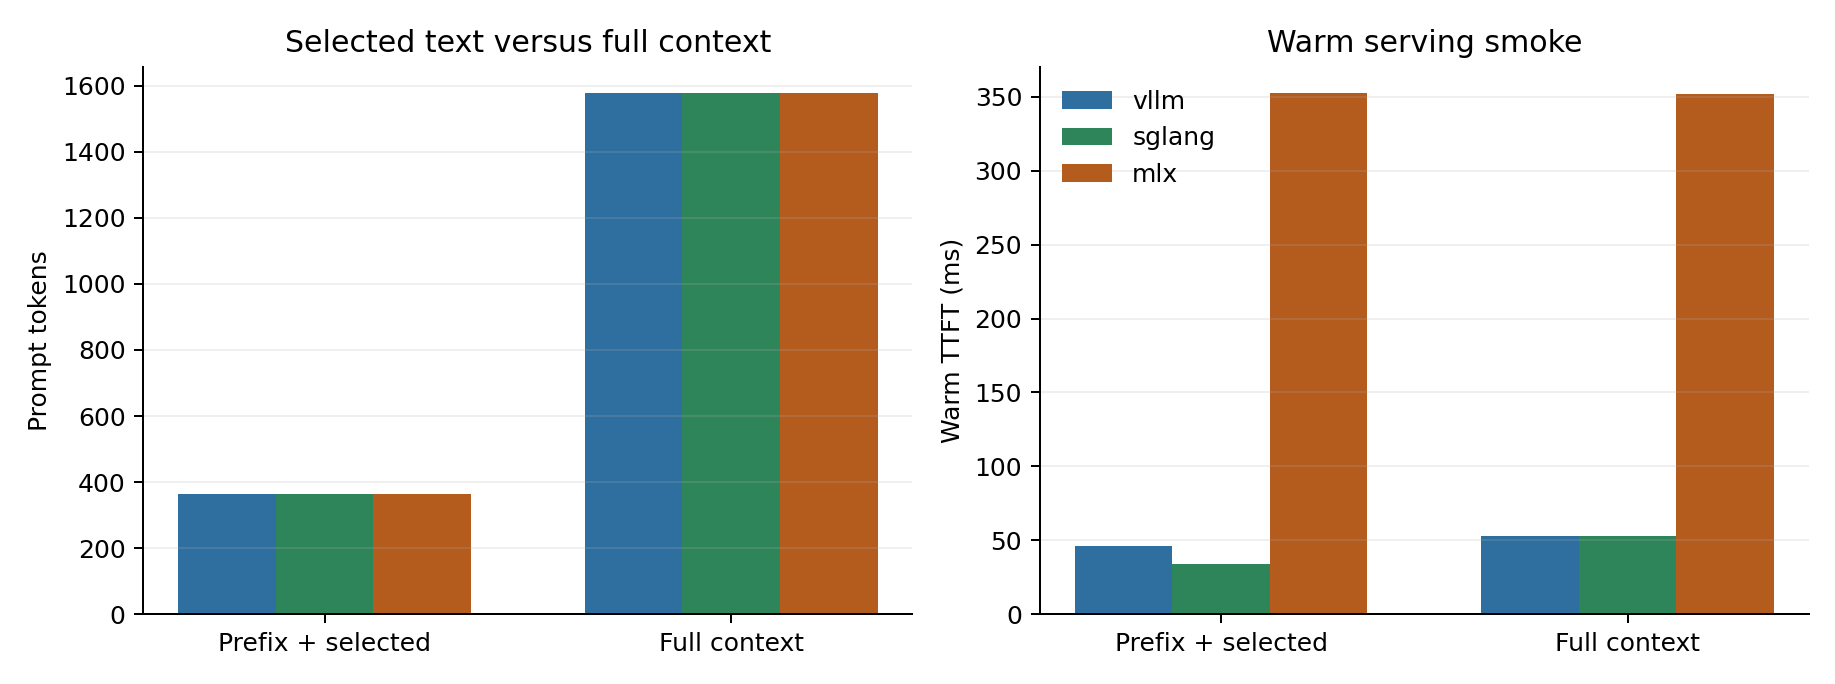
\includegraphics[width=0.98\linewidth]{../shared/results/engine_smoke_frontier.png}
\caption{Shared calibration view. Prompt sizes are identical across the Qwen
tokenizers. Absolute engine latency is not comparable because SGLang used an
unquantized model while vLLM and MLX-LM used a 4-bit checkpoint.}
\label{fig:sglang-shared}
\end{figure}

\section{Native Runner Results}
\begin{table}[t]
\centering
\small
\caption{Five-seed SGLang native-cache mechanism result. Radix separation is
the fraction for which scheduler-local length excludes selected PRA tokens.}
\begin{tabular}{rrrrr}
\toprule
Seeds & Exact & Argmax parity & Radix separation & Latency ms \\
\midrule
5 & 100\% & 100\% & 100\% & 222.0 \\ 
\bottomrule
\end{tabular}

\label{tab:sglang-native}
\end{table}

The native path recovers all five answers, preserves next-token logits exactly,
and keeps PRA tokens out of scheduler prefix length in every case. Mean
completion latency is 222.0 ms. This closes cache semantics, not hierarchy.
HiCache was disabled, so no L1/L2/L3 placement, promotion, demotion, transfer,
or reload metric exists. The SGLang MLX control plane reports no ordinary GPU
KV pool because MLX owns inference state.

The next experiment installs the bridge on the real \texttt{MlxModelRunner}.
It executes source ingestion separately, then runs selected memory through
\texttt{prefill\_start}, \texttt{prefill\_finalize}, and batched decode. Full
visible context and native memory recover 5/5 answers, while query-only disabled
memory recovers 0/5. Every native request keeps all 141 source tokens outside
the scheduler-local length.

\begin{table}[!htbp]
\centering
\small
\caption{Five-seed live-runner concurrency. One immutable selected memory is
shared by every request in a batch.}
\begin{tabular}{rrrrr}
\toprule
Concurrency & Exact & Requests/s & Shared MB saved & Scheduler isolation \\
\midrule
1 & 100\% & 6.59 & 0.0 & yes \\
2 & 100\% & 9.91 & 15.4 & yes \\
4 & 100\% & 13.25 & 46.3 & yes \\
8 & 100\% & 14.54 & 108.0 & yes \\
\bottomrule
\end{tabular}

\label{tab:sglang-live}
\end{table}

Table~\ref{tab:sglang-live} shows exact recovery at every tested concurrency.
Mean throughput rises from 6.59 requests/s at one request to 14.54 at eight,
with diminishing returns after four. Physical object sharing avoids 108.0 MiB
of duplicate selected K/V at concurrency eight. These are controlled in-process
measurements, not queued HTTP tail latency.

\subsection{Natural-text controls}
We also use balanced QASPER and HotpotQA text to build 40 examples per dataset
and condition. Each source contains an inserted \texttt{AnswerCode yes/no}
anchor among natural text. Constrained greedy decoding ranks the two answer
tokens through SGLang's own logit-edit path. This measures native transport and
causal dependence, not unrestricted benchmark QA.

\begin{table}[!htbp]
\centering
\small
\caption{SGLang live-runner natural-text transport controls.}
\begin{tabular}{llrr}
\toprule
Dataset & Condition & Samples & Ranked exact \\
\midrule
qasper & disabled & 40 & 50\% \\
qasper & native & 40 & 100\% \\
qasper & ordinary\_full & 40 & 100\% \\
qasper & shuffled & 40 & 40\% \\
hotpotqa & disabled & 40 & 50\% \\
hotpotqa & native & 40 & 100\% \\
hotpotqa & ordinary\_full & 40 & 100\% \\
hotpotqa & shuffled & 40 & 40\% \\
\bottomrule
\end{tabular}

\label{tab:sglang-natural}
\end{table}

Native and ordinary full context are 40/40 on each dataset. Disabled memory is
20/40 and shuffled memory is 16/40 on each. The negative controls establish
that successful native decisions depend on the registered source rather than
the query alone.

\begin{figure}[!htbp]
\centering
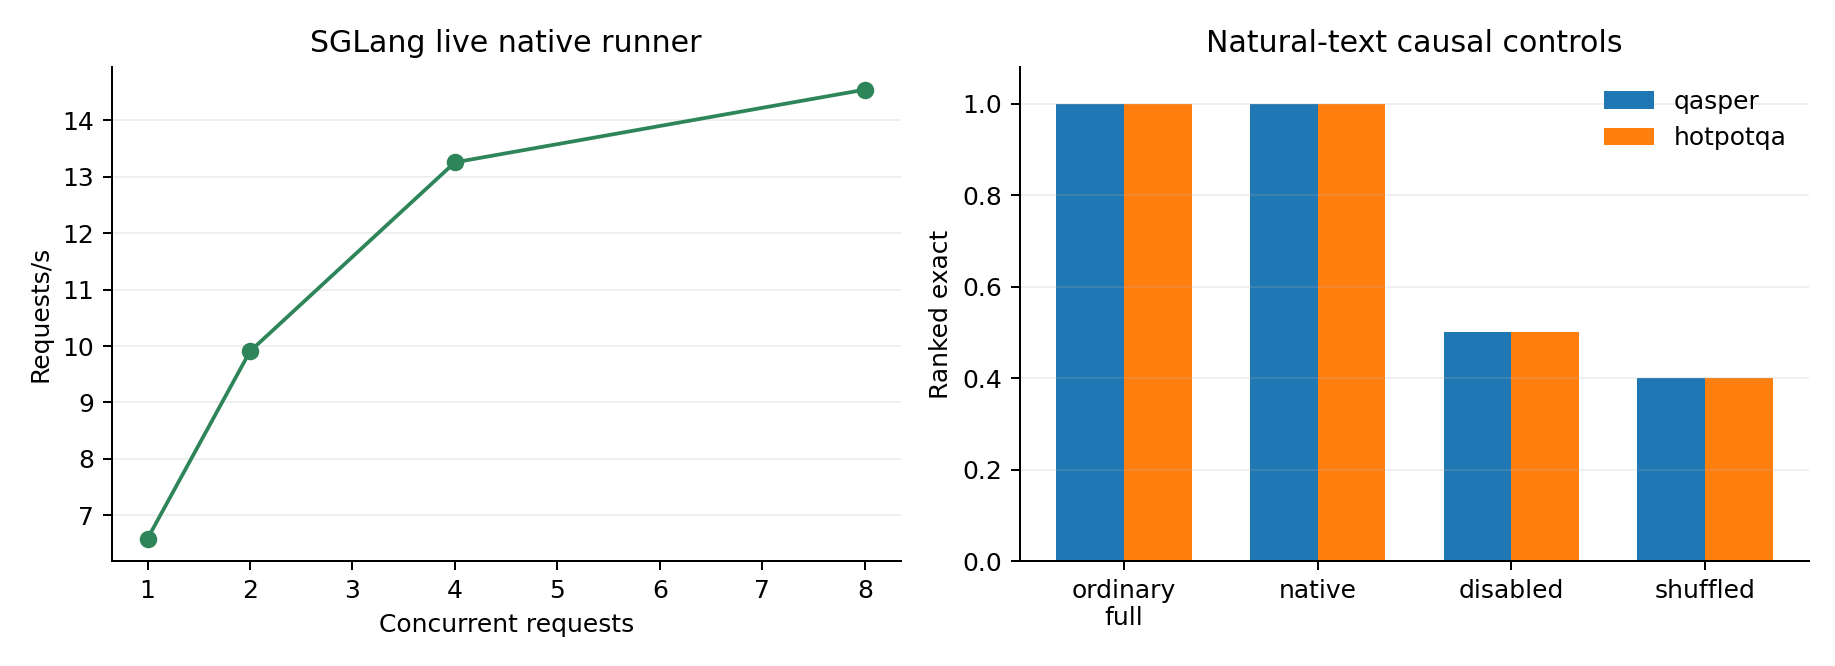
\includegraphics[width=0.98\linewidth]{../shared/results/paper6_1_sglang/live_runner_natural.png}
\caption{Live native-runner throughput and natural-text causal controls.}
\label{fig:sglang-live}
\end{figure}

\FloatBarrier
\begin{center}
\begin{tabularx}{0.96\linewidth}{l l Y}
\toprule
Gate & Status & Evidence \\
\midrule
environment & closed & patched pinned SGLang-MLX starts reproducibly \\
radix baseline & smoke closed & exact scheduler cache-token trace \\
selected-text parity & smoke closed & selected and full are 5/5 \\
HiCache non-prefix object & open & hierarchy disabled \\
selected native attention & controlled closed & 5/5 exact, zero logit error, all 28 layers \\
radix/native identity & controlled closed & PRA tokens excluded from local prefix length \\
runner lifecycle & controlled closed & prefill, batched decode, and clean request release \\
concurrency/sharing & controlled closed & five seeds at 1--8 requests; 108 MiB avoided \\
natural transport & controlled closed & native/full 80/80; causal controls near chance \\
robustness & partial & one model; synthetic and two natural-text transport fixtures \\
\bottomrule
\end{tabularx}
\end{center}

\section{Next Engine-Native Experiment}
The next useful patch moves the verified cache object into an independent
HiCache side namespace. It should place selected detail in host or unified
memory, promote it before first use, and retain the logical PRA key beside the
radix key. The matched comparison is RadixAttention plus black-box selected
text versus Radix plus native PRA at equal quality and selected-token budget.
Only then should prefetch, eviction, archived-head conversion, or cache-aware
scheduling be optimized.

\section{Falsification and Limitations}
Deep SGLang integration is unnecessary if RadixAttention plus the tuned
black-box path matches native PRA on quality-adjusted memory, TTFT, and
throughput. The current baseline is already strong, so a metadata-only object
registry cannot satisfy the claim.

The measurements use one small model family, a local compatibility patch, and
one Apple host. The HTTP and native runs use different model precisions. The
live native runner disables Radix pooling so this iteration does not yet measure
prefix and native memory inside the same scheduled request. HiCache, HTTP-level
native concurrency, tail latency, resource-affinity routing, and archived-head
transition remain unmeasured. The natural controls contain real dataset text
but an inserted answer-code task; they are not QASPER or HotpotQA end-task
scores.

\section{Related Work}
SGLang combines a structured runtime with RadixAttention for shared prefix
reuse~\cite{zheng2024sglang}. Paged serving systems manage physical KV, while
hierarchical caches extend residency across tiers. Retrieval systems select
text or documents before generation. PRA differs by assigning stable identity
to native non-prefix memory and making its active subset query dependent. The
central integration constraint is to preserve both prefix and resource
identities rather than collapse one into the other.

\section{Conclusion}
On the pinned SGLang-MLX environment, selected context and RadixAttention are
clearly complementary: the selected condition preserves 5/5 recovery, removes
76.9\% of visible prompt tokens, and reuses 364 of 365 tokens on warm requests.
The native SGLang-cache path additionally gives 5/5 recovery and exact logit
parity without adding PRA tokens to Radix prefix length. The live runner keeps
that result through batched decode, scales to 14.54 requests/s at concurrency
eight, and passes 80/80 natural-text transport decisions while disabled and
shuffled controls fall near chance. SGLang attention can therefore consume
selected non-prefix K/V while preserving the two address spaces. Paper 6.1
leaves HiCache placement, combined Radix-plus-native scheduling, and
pressure-scale server validation as the focused next experiments.

\begin{thebibliography}{9}
\bibitem{zheng2024sglang}
L. Zheng et al.
\newblock SGLang: Efficient Execution of Structured Language Model Programs.
\newblock 2024.
\end{thebibliography}

\end{document}
